% ============================================
% SEZIONE 10: EXPLAINABLE AI (XAI)
% ============================================

\section{Explainable AI}
\label{sec:explainability}

L'interpretabilit\`a dei modelli di deep learning \`e fondamentale per comprendere \textit{cosa} il modello ha imparato e identificare potenziali bias nei dati. Questa sezione presenta l'analisi XAI condotta sui quattro classificatori di ResQPet.

\subsection{Motivazione}

I modelli di deep learning sono spesso considerati ``black box'': producono predizioni accurate ma senza spiegare il ragionamento sottostante. Le tecniche di Explainable AI permettono di:
\begin{itemize}
    \item \textbf{Validare} che il modello utilizzi features semanticamente corrette
    \item \textbf{Identificare} bias nei dati di training
    \item \textbf{Debuggare} comportamenti inattesi
    \item \textbf{Costruire fiducia} negli utenti finali del sistema
\end{itemize}

\subsection{Tecniche Utilizzate}

\begin{table}[H]
\centering
\begin{tabular}{llp{6cm}}
\toprule
\textbf{Modello} & \textbf{Tecnica XAI} & \textbf{Descrizione} \\
\midrule
Breed Classifier & GradCAM++ & Gradient-weighted Class Activation Mapping per CNN \\
Collar Detector & Feature Attention Maps & Mappe di attivazione dal backbone YOLO \\
Backbone YOLO11 & Keypoint Reliability & Analisi confidenza per punto anatomico \\
Pose Classifier & SHAP & SHapley Additive exPlanations per MLP \\
\bottomrule
\end{tabular}
\caption{Tecniche XAI applicate a ciascun modello.}
\label{tab:xai_techniques}
\end{table}

\subsection{Breed Classifier: GradCAM++}

GradCAM++ \cite{chattopadhay2018gradcam} genera heatmap che evidenziano le regioni dell'immagine pi\`u influenti per la predizione. Per il Breed Classifier (EfficientNet-B0), l'analisi ha confermato che il modello:
\begin{itemize}
    \item Focalizza l'attenzione sulla \textbf{testa} del cane (forma del muso, orecchie)
    \item Considera la \textbf{struttura corporea} generale
    \item Ignora correttamente lo sfondo e elementi irrilevanti
\end{itemize}

\begin{figure}[H]
    \centering
    \includegraphics[width=\textwidth]{figures/breed_xai_multi_image.png}
    \caption{Analisi GradCAM++ del Breed Classifier su diverse immagini. La riga superiore mostra le immagini originali, quella inferiore le heatmap di attivazione. Le zone calde (rosso/giallo) indicano le regioni pi\`u influenti per la classificazione della razza.}
    \label{fig:breed_xai}
\end{figure}

Questo comportamento \`e semanticamente corretto: la razza canina \`e determinata principalmente da caratteristiche morfologiche del muso e della struttura corporea.

\subsection{Collar Detector: Analisi Critica}
\label{sec:collar_bias}

L'analisi XAI del Collar Detector ha rivelato un \textbf{potenziale dataset bias} significativo.

\subsubsection{Metodologia}

Sono state estratte le Feature Attention Maps dal backbone YOLOv8n utilizzando forward hooks sui layer convoluzionali. Le mappe di attivazione mostrano quali regioni dell'immagine il modello considera per la detection.

\subsubsection{Finding Critico}

\begin{figure}[H]
    \centering
    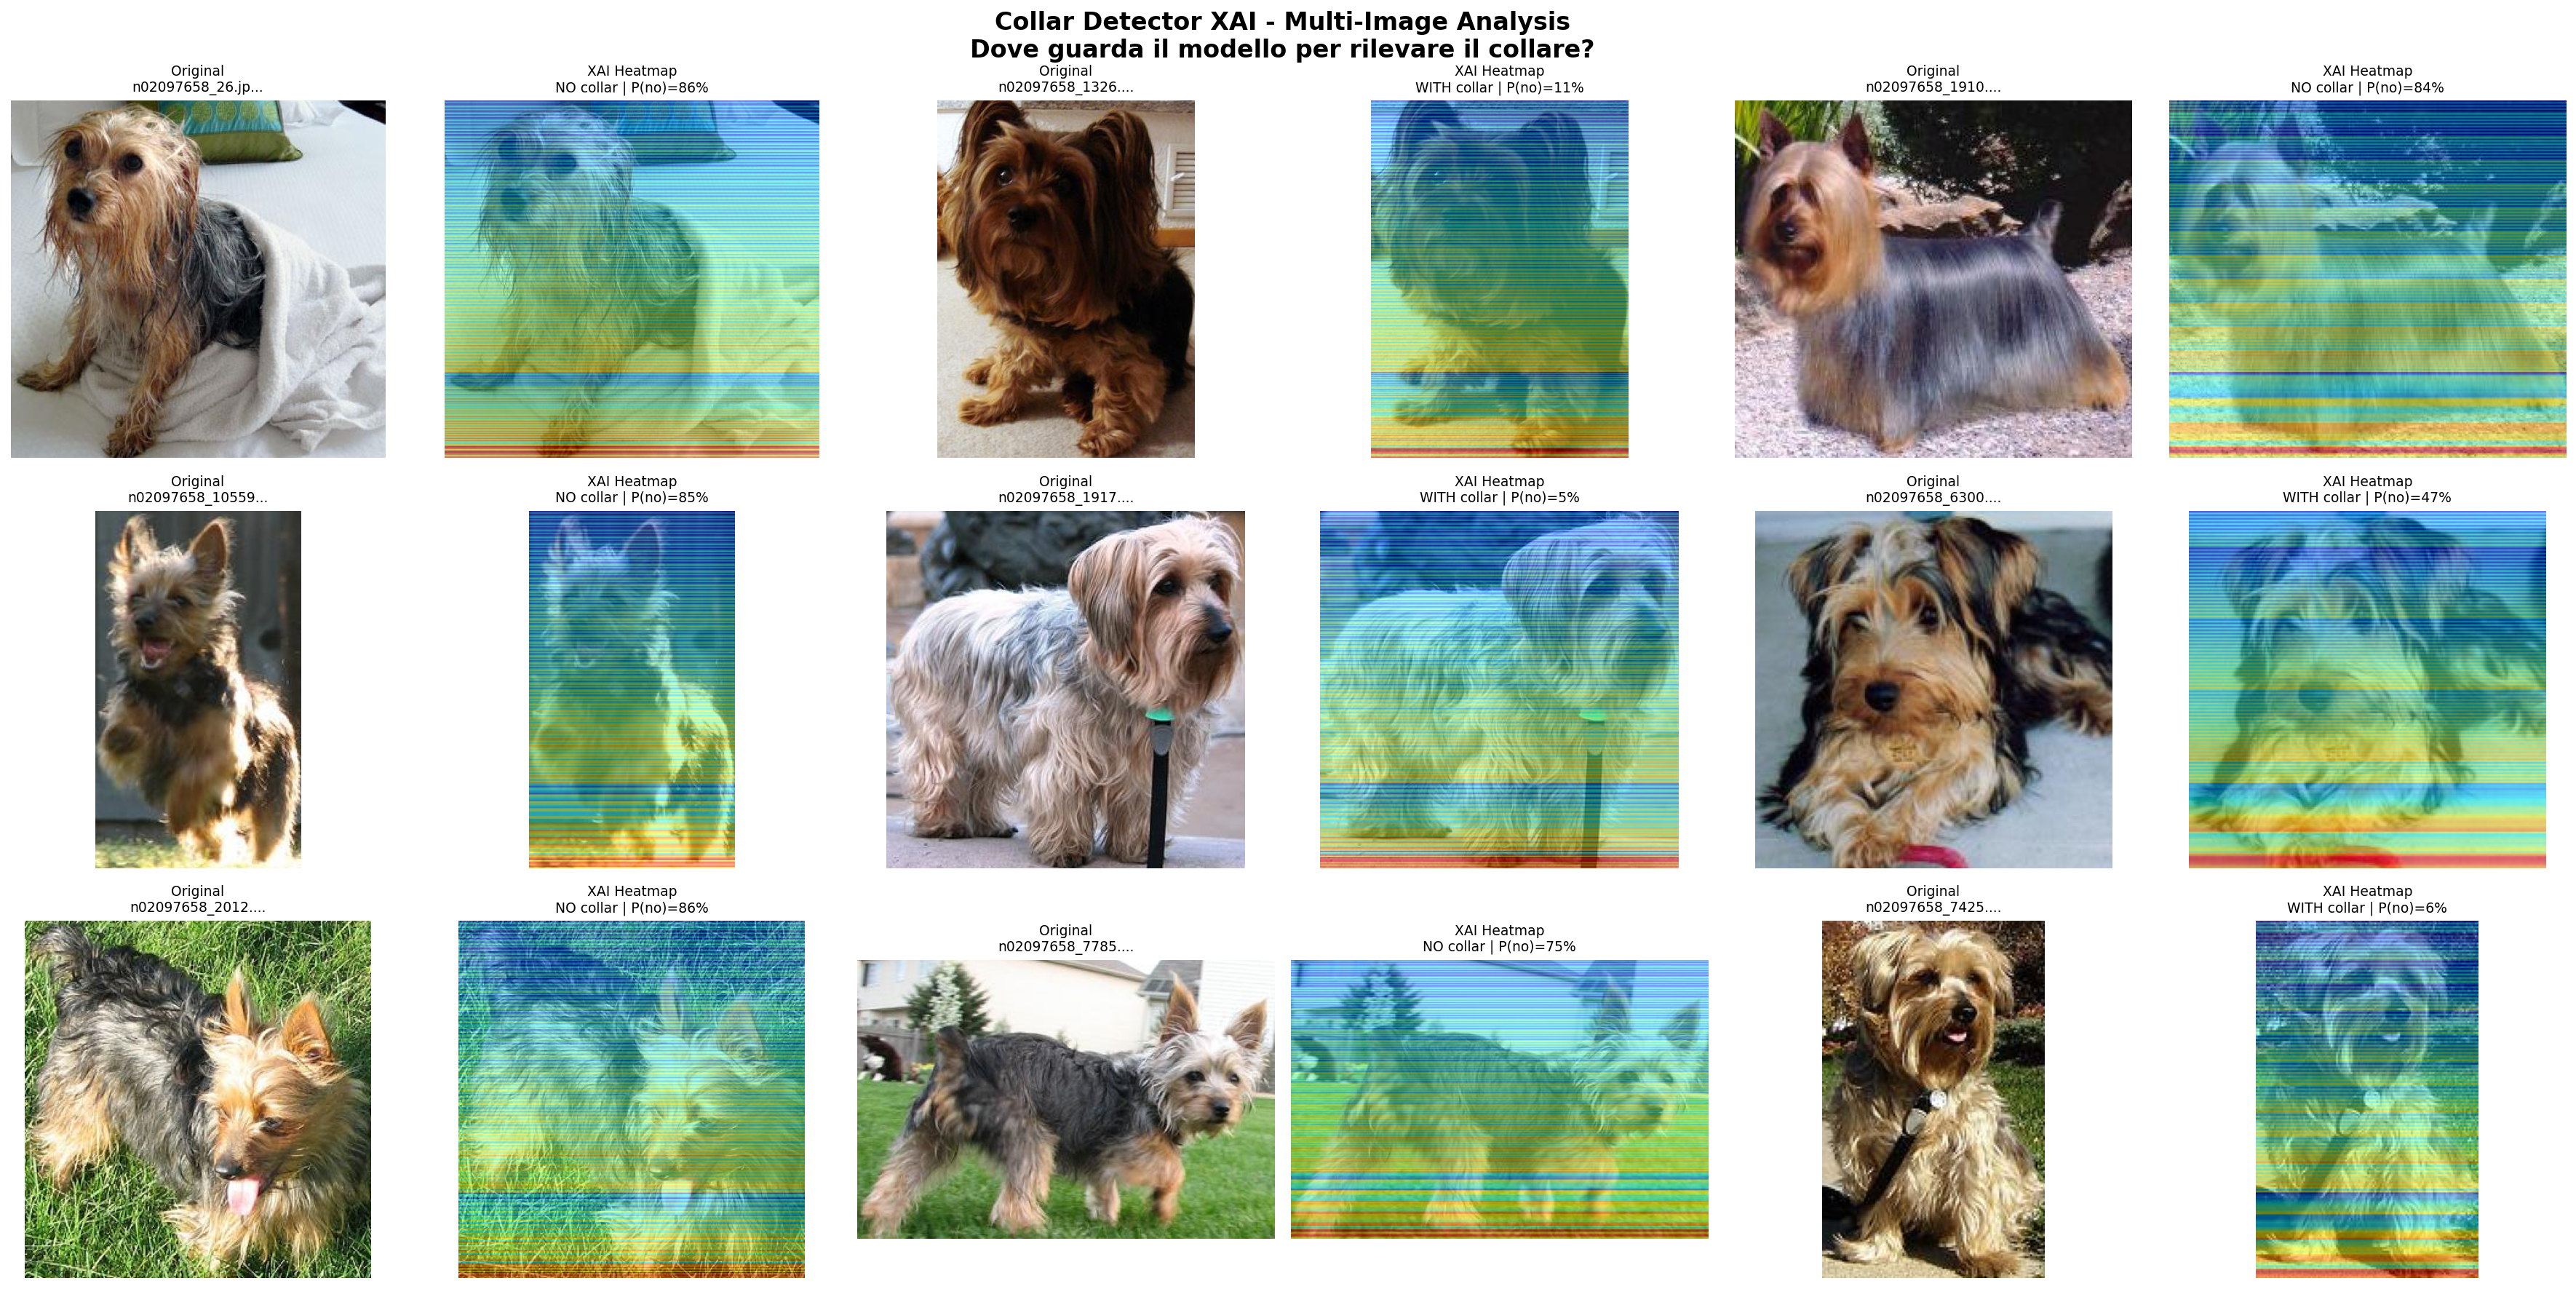
\includegraphics[width=\textwidth]{figures/collar_xai_multi_image.png}
    \caption{Analisi XAI del Collar Detector su diverse immagini. Per ogni coppia: immagine originale (sinistra) e heatmap di attenzione (destra). \textbf{Osservazione critica}: le zone calde sono spesso concentrate sulla parte inferiore dell'immagine (pavimento/erba) invece che sulla regione del collo.}
    \label{fig:collar_xai}
\end{figure}

\paragraph{Interpretazione:} Questo suggerisce che il modello potrebbe aver appreso \textbf{correlazioni spurie} dal dataset:
\begin{itemize}
    \item I cani \textbf{con collare} nel dataset potrebbero essere prevalentemente fotografati su superfici specifiche (es. pavimento domestico, marciapiede)
    \item I cani \textbf{senza collare} potrebbero essere prevalentemente in contesti diversi (es. erba, terra battuta)
    \item Il modello ha imparato a predire la presenza del collare basandosi sullo \textbf{sfondo} invece che sul collare stesso
\end{itemize}

\subsubsection{Analisi GradCAM Class-Specific}

Per confermare l'ipotesi del bias, \`e stata condotta un'analisi GradCAM separata per ciascuna classe di output, utilizzando la libreria \texttt{pytorch-grad-cam}.

\begin{figure}[H]
    \centering
    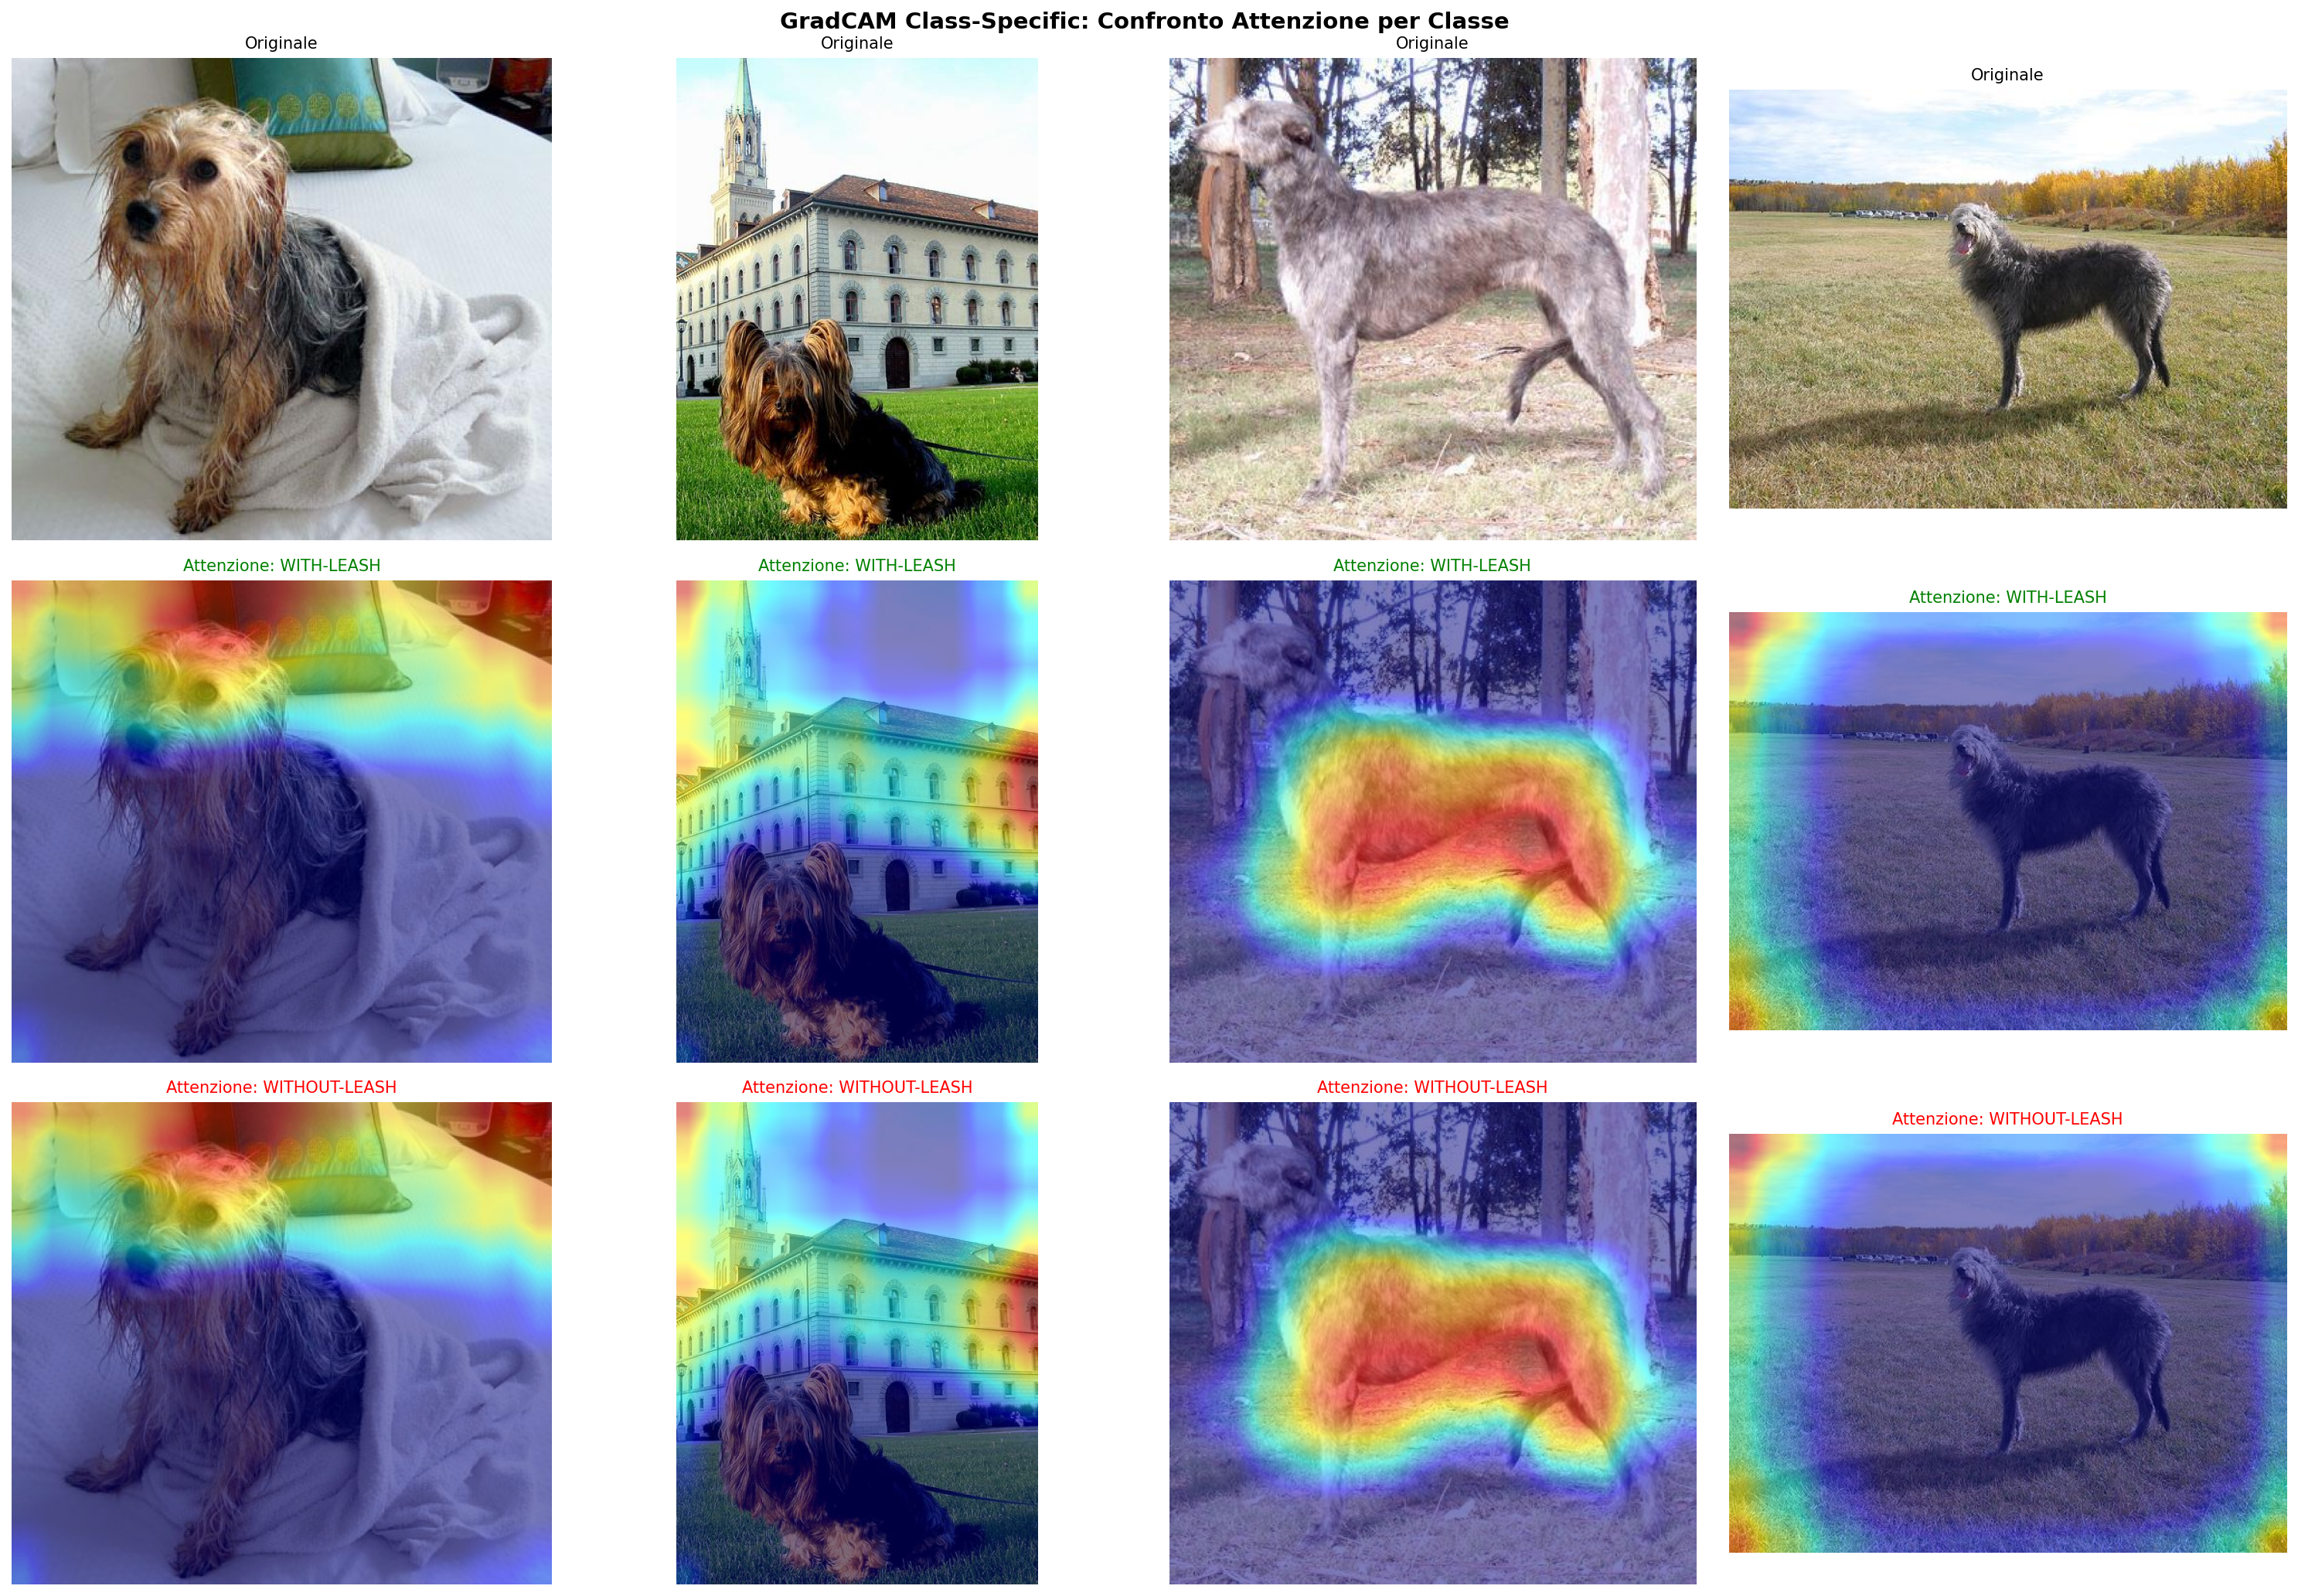
\includegraphics[width=\textwidth]{figures/collar_gradcam_class_comparison.png}
    \caption{Confronto GradCAM class-specific su immagini Stanford Dogs. Riga 1: immagini originali. Riga 2: mappa di attenzione per classe ``Dog-with-Leash''. Riga 3: mappa di attenzione per classe ``Dog-without-Leash''. Le heatmap sono \textbf{quasi identiche} tra le due classi.}
    \label{fig:collar_gradcam_comparison}
\end{figure}

\paragraph{Risultato Critico:} L'analisi class-specific rivela un problema fondamentale:

\begin{itemize}
    \item Le mappe di attenzione per \textbf{entrambe le classi sono identiche}
    \item L'attenzione \`e concentrata sul \textbf{corpo centrale} del cane, non sulla regione del collo
    \item Il modello non mostra \textbf{nessuna differenza} nel pattern di attenzione tra ``cercare il collare'' e ``verificare l'assenza del collare''
\end{itemize}

\paragraph{Interpretazione:} Un Collar Detector correttamente addestrato dovrebbe mostrare:
\begin{itemize}
    \item Per \textbf{Dog-with-Leash}: focus sulla zona \textbf{collo/collare}
    \item Per \textbf{Dog-without-Leash}: focus sulla zona \textbf{collo} per verificarne l'assenza
\end{itemize}

Il fatto che le heatmap siano identiche suggerisce che la decisione di classificazione avviene basandosi su \textbf{features non discriminative} (probabilmente correlazioni spurie con lo sfondo o il contesto), confermando il dataset bias ipotizzato.

\subsubsection{Implicazioni}

Nonostante il Collar Detector raggiunga un mAP@0.5 di 0.853 sul validation set, questo finding solleva dubbi sulla \textbf{generalizzazione} del modello:
\begin{itemize}
    \item Il modello potrebbe fallire su immagini dove lo sfondo non correla con la presenza del collare
    \item In deployment reale, le condizioni ambientali potrebbero differire significativamente dal training set
    \item \`E necessario un dataset pi\`u bilanciato in termini di contesti/sfondi
\end{itemize}

\paragraph{Azione Correttiva Proposta:} Per le versioni future, si propone di:
\begin{enumerate}
    \item Aumentare la variet\`a di sfondi nel dataset di training
    \item Applicare augmentation pi\`u aggressivo sullo sfondo (random background replacement)
    \item Utilizzare tecniche di object-centric learning per forzare l'attenzione sulla regione del collo
\end{enumerate}

\subsection{Backbone YOLO11: Keypoint Reliability}

Per il backbone di pose estimation, l'analisi si \`e concentrata sulla \textbf{affidabilit\`a dei keypoints} per gruppo anatomico.

\subsubsection{Analisi per Gruppo Anatomico}

I 24 keypoints sono stati raggruppati in categorie anatomiche:

\begin{figure}[H]
    \centering
    \includegraphics[width=\textwidth]{figures/backbone_keypoint_reliability.png}
    \caption{Analisi dell'affidabilit\`a dei keypoints. A sinistra: distribuzione della confidenza media per keypoint. A destra: matrice di correlazione tra gruppi anatomici.}
    \label{fig:backbone_reliability}
\end{figure}

\begin{table}[H]
\centering
\begin{tabular}{lcc}
\toprule
\textbf{Gruppo} & \textbf{Keypoints} & \textbf{Confidenza Media} \\
\midrule
Testa (nose, eyes, ears) & 5 & Alta ($> 0.8$) \\
Torso (withers, throat, tailbase) & 3 & Alta ($> 0.75$) \\
Zampe anteriori & 8 & Media ($\sim 0.6$) \\
Zampe posteriori & 8 & Media ($\sim 0.55$) \\
\bottomrule
\end{tabular}
\caption{Affidabilit\`a media dei keypoints per gruppo anatomico.}
\label{tab:keypoint_reliability}
\end{table}

\paragraph{Osservazioni:}
\begin{itemize}
    \item I keypoints della \textbf{testa} sono i pi\`u affidabili (sempre visibili)
    \item Le \textbf{zampe} hanno confidenza pi\`u variabile (occlusioni frequenti)
    \item Il Pose Classifier \`e robusto a queste variazioni grazie alla normalizzazione dei keypoints
\end{itemize}

\subsection{Pose Classifier: SHAP Analysis}

SHAP (SHapley Additive exPlanations) \cite{lundberg2017shap} fornisce spiegazioni a livello di feature per modelli tabellari come l'MLP del Pose Classifier.

\subsubsection{Features pi\`u Influenti}

L'analisi SHAP ha identificato le features pi\`u discriminanti per la classificazione stray/owned:

% Figura SHAP non disponibile - analisi testuale inclusa sotto
% \begin{figure}[H]
%     \centering
%     \includegraphics[width=\textwidth]{figures/pose_xai_multi_image.png}
%     \caption{Visualizzazione SHAP del Pose Classifier.}
%     \label{fig:pose_xai}
% \end{figure}

\begin{enumerate}
    \item \textbf{Posizione relativa della coda} (tailbase\_y normalizzato)
    \item \textbf{Apertura delle zampe posteriori} (distanza tra back\_left\_paw e back\_right\_paw)
    \item \textbf{Postura della testa} (nose\_y rispetto a withers\_y)
\end{enumerate}

\paragraph{Interpretazione:}
\begin{itemize}
    \item Coda bassa/tra le zampe $\rightarrow$ indica stress/paura (comune nei randagi)
    \item Zampe ravvicinate $\rightarrow$ postura difensiva
    \item Testa abbassata $\rightarrow$ sottomissione o ricerca di cibo
\end{itemize}

Questi pattern sono coerenti con la letteratura sul comportamento canino \cite{overall2013canine}, validando l'approccio weak supervision.

\subsection{Riepilogo e Raccomandazioni}

\begin{table}[H]
\centering
\begin{tabular}{lcp{5cm}}
\toprule
\textbf{Modello} & \textbf{XAI Status} & \textbf{Azione Raccomandata} \\
\midrule
Breed Classifier & \checkmark Corretto & Nessuna \\
Collar Detector & $\times$ \textbf{Bias grave} & Retraining con dataset bilanciato e ROI cropping su zona collo \\
Backbone YOLO11 & \checkmark Corretto & Nessuna \\
Pose Classifier & \checkmark Corretto & Nessuna \\
\bottomrule
\end{tabular}
\caption{Riepilogo analisi XAI e azioni raccomandate.}
\label{tab:xai_summary}
\end{table}

\paragraph{Conclusione:} L'analisi XAI ha rivelato che tre modelli su quattro utilizzano features semanticamente appropriate. Il \textbf{Collar Detector presenta un bias critico} confermato dall'analisi GradCAM class-specific: le mappe di attenzione identiche per entrambe le classi indicano che il modello non ha appreso a distinguere la presenza/assenza del collare guardando la regione anatomica corretta. Nonostante le buone metriche sul validation set (mAP 0.853), questo finding solleva seri dubbi sulla generalizzazione del modello in scenari reali. L'analisi XAI si \`e dimostrata fondamentale per identificare questo problema, che non sarebbe emerso dalle sole metriche quantitative.

